\documentclass[titlepage]{article}

\usepackage[utf8]{inputenc}
\usepackage[dutch]{babel}
\usepackage{parskip}
\usepackage{a4wide}
\usepackage{amsmath}

\usepackage{graphicx}
\usepackage{float}
\usepackage{subcaption}
\usepackage{placeins}
\graphicspath{ {images/} }

\DeclareMathOperator*{\argmin}{arg\,min}

\newenvironment{note}{\textbf{Opmerking}}{}

\title{Project Beeldverwerking}
\author{Yasser {Deceukelier} \and Bart {Middag} \and Tituoan {Vervack} }
\date{}

\begin{document}

\maketitle

\section{Herkenning opvulgebied}

\begin{note}
Voor deze opgave maken we gebruik van het bestand \texttt{magicwand.m}. Dit is een functie die in een afbeelding voor een gegeven pixel alle aangrenzende pixels met een gelijkaardige kleurwaarde selecteert (zoals de magic wand tool in Photoshop bijvoorbeeld). Deze code komt van Matlab central.
\end{note}

Ons algoritme hiervoor werkt in twee stappen:
\begin{enumerate}
\item 
Eerst doorlopen we de afbeelding op zoek naar een gele pixel. Als we een gele pixel tegen komen, gebruiken we de \verb!magicwand! functie om alle aangrenzende pixels met exact dezelfde kleur te vinden. We berekenen een score voor deze groep van pixels en tellen die op in een histogram per kleur. Er wordt voor gezorgd dat we elke pixel slechts een maal in rekening brengen. Het resultaat is een histogram, waarin voor elk kleur een score gebaseerd op het aantal aangrenzende pixel met dezelfde kleur opgeslagen is. 
\par
We gaan er van uit dat deze score het grootst zal zijn voor de aangebrachte markeringen, aangezien deze met een computer zijn aangebracht en elke pixel van de markering exact dezelfde kleur zal hebben. Uit het histogram nemen we dan de kleur met de meeste aangrenzende pixels en veronderstellen dat dit het markeringskleur is.
\item
In de tweede fase overlopen we de afbeelding nogmaals, zoeken we elke pixel met de markeringskleur en voegen die toe aan het masker. Het masker is echter niet accuraat aan de randen van de markeringen. Daarom gaan we voor elke pixel die deel uitmaakt van het masker alle 9 omliggende pixels ook toevoegen aan het masker. Dit is een vrij eenvoudige oplossing, maar ze blijkt vrij doeltreffend te zijn.
\end{enumerate}

\section{Opvullen van ontbrekende gebieden}
\subsection{Rekencomplexiteit}
De rekencomplexiteit van dit algoritme is $\mathcal{O}\left(S^2 \times \left(I + (B^2 \times n)\right)\right)$. Hierbij is $n$ het aantal ontbrekende pixelintensiteiten, $S$ de grootte van het zoekvenster (met $S^2$ het aantal pixels in het zoekvenster) en $B$ de blokgrootte. $I$ is het totale aantal pixels in het beeld -- we overlopen immers het volledige beeld om de ontbrekende pixelintensiteiten te vinden.\\
Het exacte aantal operaties is gelijk aan $(S^2-1)  \times (I + (B^2  \times 5 + 1)  \times n)$. In het geval van 50000 ontbrekende pixelintensiteiten, een zoekvenster van 400x400 en een blokgrootte van 12x12 wordt dit:
\begin{equation*}
(400^2-1)  \times (1000000 + (12^2  \times 5 + 1) \times 50000) = 5927962950000
\end{equation*}

\subsection{Verbetering met integraalvoorstelling} \label{integraalvoorstelling}
Met de integraalvoorstelling kunnen we de complexiteit van deze formule sterk verminderen. De formule ziet er nu als volgt uit:
\begin{equation*} \widehat{y(m,n)} = \begin{cases}
	y(m,n)
    	& \text{als $\alpha(m,n) = 1$}  \\
	\begin{aligned} 
	& y((m,n) + \argmin_{(\Delta m, \Delta n) \in S} \frac{1}{B^2} \times \\
    \Big( & F_{\Delta m,\Delta n}(m+b,n+b) - F_{\Delta m,\Delta n}(m+b,n-b) \\
    - & F_{\Delta m,\Delta n}(m-b,n+b) + F_{\Delta m,\Delta n}(m-b,n-b) \Big)
    \end{aligned}
    	& \text{als $\alpha(m,n) = 0$}
   \end{cases}
\end{equation*}
Hierbij is $b$ gelijk aan $\dfrac{B}{2}$. \\ \\

De rekencomplexiteit van het verbeterde algoritme is $\mathcal{O}\left(S^2 \times \left(I + n)\right)\right)$. Nu we de integraalvoorstelling van het beeld berekenen gebeurt de berekening van de som over een blok immers in constante tijd.\\
Het exacte aantal operaties is gelijk aan $(S^2-1)  \times (5 \times I + 4 \times n)$. In het geval van 50000 ontbrekende pixelintensiteiten, een zoekvenster van 400x400 en een blokgrootte van 12x12 wordt dit:
\begin{equation*}
(400^2-1)  \times (5 \times 1000000 + 4 \times 50000) = 831994800000
\end{equation*}
In dit geval zal het algoritme dus $7.125$ keer zo snel zijn als een brute-force implementatie. Met grotere blokgrootte zal het effect nog groter zijn.

\subsection{Implementatie in MATLAB}
Tijdens de implementatie in MATLAB werd het algoritme aangepast om inpainting bij de randen van het beeld te ondersteunen. Hiervoor werden de randpixels gebruikt om een extra rand van $\frac{B}{2}$ pixels op te vullen. \\
Ook werd de formule aangepast zodat ze geen voorkeur meer gaf aan blokken waar er meer onbekende pixels waren.
Door deze aanpassingen is het exacte aantal operaties hoger dan beschreven in sectie  \ref{integraalvoorstelling}, maar de complexiteit blijft onveranderd. \\
De formule zonder integraalvoorstelling werd eveneens ge\"implementeerd en geeft dezelfde resultaten.

\subsection{Probleem bij MSD}
Zoals in de vorige vraag al is vermeld is het probleem dat blokken met veel onbekende pixels bevoordeeld werden, terwijl dit natuurlijk het omgekeerde is van wat we willen bereiken. Dit is omdat er gedeeld werd door $B^2$ (de gehele blokgrootte) bij het berekenen van de MSD, hoewel er in vele gevallen minder pixels gebruikt werden. Hiervoor werd de integraalvoorstelling van de matrix $\alpha_{\Delta m,\Delta n}(m,n) = \alpha(m,n) \times \alpha(m+\Delta m, n+\Delta n)$ berekend.

\subsection{Opvullen in iteraties} \label{slicing}
Hoewel we nu geen voorkeur meer geven aan blokken met veel ontbrekende pixels, probeert de formule nog steeds zo veel mogelijk pixels op te vullen: zolang 1 pixel bekend is in de blok gecentreerd rond de in te painten pixel en met een andere pixel in het zoekvenster kan vergeleken worden, zal de pixel ingepaint worden.\\
Om dit op te lossen, berekenen we aan het begin van elke iteratie de integraalvoorstelling van het Mask om het aantal gekende pixels in de blok gecentreerd rond elke in te painten pixel te bepalen. Enkel de pixels met het maximale aantal gekende pixels (of binnen een factor \texttt{slicing\char`_factor} van dit maximum) in de buurt worden ingepaint in de daarop volgende iteratie.\\ \\
Hoewel het algoritme veel trager wordt door het toevoegen van iteraties, zou het hiermee betere resultaten moeten produceren. Dit is echter niet altijd het geval, doordat hiermee in plaats van de oorspronkelijke pixels meer ingepainte pixels gebruikt worden om andere pixels in te painten. Het is dus een uitdaging om een goede factor \texttt{slicing\char`_factor} te vinden waarmee het algoritme genoeg pixels per iteratie probeert in te painten, maar niet te veel.

\subsection{Verbetering met mathematische morfologie} \label{erosie}
We kunnen erosie toepassen op de blokken met onbekende pixels om zo het aantal blokken met veel onbekende pixels te verkleinen. In MATLAB implementeren we dit door lijn per lijn op zoek te gaan naar lijnen met onbekende pixels, deze selecteren we dan en padden we dan met de $\frac{B}{2}$ pixels langs elke kant. Op deze lijn passen we erosie toe indien de eerste pixel en de laatste pixel niet te veel verschillen in kleur. Dit doen we om artefacten bij grote kleursveranderingen tegen te gaan.
Het toepassen van erosie op deze manier heeft niet zo een groot effect, het enige dat opvalt is dat de randen van de opgevulde stukken nu iets minder zichtbaar zijn waardoor het opgevulde deel iets minder opvalt.

\subsection{Vaststellingen en verbeteringen}
Tot nu toe staven de resultaten van onze methode met de verwachtingen: het algoritme slaagt erin om ontbrekende pixels goed in te painten. Op vlak van berekeningstijd presteert het algoritme echter minder goed.\\ \\
Dit ligt vooral aan het algoritme uit sectie \ref{slicing}. Het is moeilijk om voor dit algoritme parameters te vinden die voor elk beeld noch te weinig, noch te veel pixels inpaint per iteratie. Met de erosie uit sectie \ref{erosie} kunnen we dit verbeteren. We passen erosie aan het begin van elke iteratie toe op het masker om de buitenkant van elke ontbrekende ruimte te markeren, die we dan inpainten. Zo heeft het algoritme minder iteraties nodig zonder de voordelen van de aanpak met iteraties te verliezen.

\section{Ruis} % (fold)

\subsection{Invloed van ruis} % (fold)
We gaan er van uit dat de gele markeringen aangebracht worden na toevoeging van ruis. Daarom detecteren we eerst de markeringen op de originele afbeelding, daarna voegen we ruis toe en passen we het inpaintingsalgoritme toe.
We zien dat het toevoegen van ruis geen opvallend negatief effect heeft, toch niet voor de menselijke waarnemer. Inpainting op de originele afbeelding vertoont hier en daar een paar artifacten: bijvoorbeeld een paar pixels die een afwijkende kleur hebben. Door het invoeren van ruis zullen de pixelwaarden over het hele beeld wat afwijken; hierdoor vallen de artefacten van het inpaintingsalgoritme minder op. Hoger ruisniveaus verbergen deze artefacten dan ook beter dan lagere. 

% subsection invloed_van_ruis (end)

\subsection{Blokgroottes} % (fold)
Bij grote hoeveelheden ruis, zullen kleinere blokgroottes slechter presteren. We gaan namelijk op zoek naar een zo gelijkaardig mogelijk blok. Door de ge\"introduceerde ruis kunnen 2 blokken, die in de originele afbeelding niet gelijkaardig zijn, toch een zeer kleine MSD hebben waardoor deze gekozen worden om ontbrekende pixels te reconstrueren. Als 2 blokken met meer pixels worden vergeleken is de kans kleiner dat deze door willekeurig ruis allemaal gelijkaardig zijn. Bij grote blokken zal de kans op een lage MSD door de toegevoegde ruis dus kleiner zijn, omdat de ruis op verschillende pixels elkaar (gedeeltelijk) zal uitmiddelen. Hierdoor zullen de blokken die in de originele afbeelding gelijkaardig waren ook grotere kans hebben op een lage MSD.
% subsection blokgroottes (end)

\subsection{Kandidaten} % (fold)
\label{kandidaten}
Een mogelijkheid om de invloed van ruis op de MSD te beperken is door de gemiddelde waarde van een pixel en zijn naburige pixels te nemen en deze te vergelijken. De ge\"introduceerde ruistermen van naburige pixels kunnen elkaar mogelijk compenseren. De formules vermeld in \ref{integraalvoorstelling} blijven hetzelfde, behalve $f_{\Delta m, \Delta n}(m,n)$ waarin $y(m,n)$ vervangen wordt door $y_a(m,n)$ die de pixelwaarde $y(m,n)$ uitmiddelt met de $(a+1)^2$ naburige pixels.
\begin{subequations}
\begin{equation*}
	f_{\Delta m, \Delta n}(m,n) = |y_a(m+k,n+l) - y_a(m+k+\Delta m, n+l+\Delta n)|^2
\end{equation*}
\text{Met $y_a(m,n)$ gedefini\"eerd als volgt:}
\begin{equation*}
	y_a(m,n) = \frac{\sum_{i=-a}^{a} \sum_{j=-a}^{a} y'(m+i,n+j) * \alpha(m+i,n+j)}{\sum_{i=-a}^{a} \sum_{j=-a}^{a} \alpha(m+i,n+j)}
\end{equation*}
\text{waarbij}
\begin{equation*}
	y'(m,n) = \begin{cases}
		y(m,n) &\text{als $(m,n)$ binnen de grenzen van de afbeelding valt} \\
		0 &\text{anders} 	 \\
	\end{cases}
\end{equation*}
\end{subequations}
en waarbij $\alpha(m,n)$ het binaire masker is. $\alpha(m,n)$ is ook nul voor waarden $(m,n)$ die buiten de afbeelding vallen.
\par
Bij het gebruik van deze metriek blijken grotere blokgroottes beter te presteren. Dit is waarschijnlijk te wijten aan het feit dat meer informatie in rekening wordt gebracht, omdat meer uitgemiddelde pixels worden bekeken om een betere match te vinden.

% subsection kandidaten (end)

\subsection{Ruisonderdrukking en inpainting} % (fold)
\label{ruisonderdrukking_en_inpaintig}
\begin{note}
De ruisonderdrukking na het inpainten in deze opgave gebeurt met een bilaterale filter, die zorgt dat de ruis grotendeels uitgemiddeld wordt terwijl de randen bewaard blijven. Hiervoor maken we gebruik van het bestand \texttt{bfilter2.m}. Deze code komt van MatLab Central.
\end{note}

Er bestaan verschillende mogelijke strategie\"en om inpainting en ruisonderdrukking samen te gebruiken.

\'E\'en ervan is het toepassen van ruisonderdrukking voor inpainting. Zo zou de berekening van de MSD minder be\"invloed worden door ruiswaarden. Eventuele artefacten die toegevoegd worden door inpainting blijven echter achter in het resultaat.\\
Een andere strategie is het toepassen van ruisonderdrukking na inpainting. De berekening van de MSD wordt wel be\"invloed door ruiswaarden, maar artefacten die toegevoegd worden door inpainting worden over het algemeen uitgemiddeld door de ruisonderdrukking.

Zoals beschreven in sectie \ref{kandidaten} proberen we de voordelen van beide strategie\"en te combineren door eerst ruisonderdrukking toe te passen bij de berekening van de MSD en dan opnieuw na het inpainten. Op figuur \ref{fig:lincoln_medium} zien we echter dat het resultaat niet overeenkomt met onze initi\"ele verwachtingen: het algoritme zonder ruisonderdrukking tijdens de berekening van de MSD presteert nog steeds schijnbaar beter. De artefacten door de invloed van ruis op de MSD zijn hier namelijk klein en worden dus samen met de ruis weggewerkt. Als we ruisonderdrukking toepassen bij de berekening van de MSD selecteert het algoritme referentiepixels gebaseerd op hun uitgemiddelde waarde -- maar dit kan een ruispixel zijn in de oorspronkelijke figuur. In volgende iteraties wordt deze ruispixel gemakkelijk uitgebreid, dus het is belangrijk om te voorkomen dat een ruispixel gekozen wordt. Dit gebeurde voordien minder gemakkelijk omdat dergelijke ruispixels de MSD sterk verhoogden.

\begin{figure}[H]
\centering
\begin{subfigure}[b]{\linewidth}
	\centering
    \captionsetup{justification=centering}
    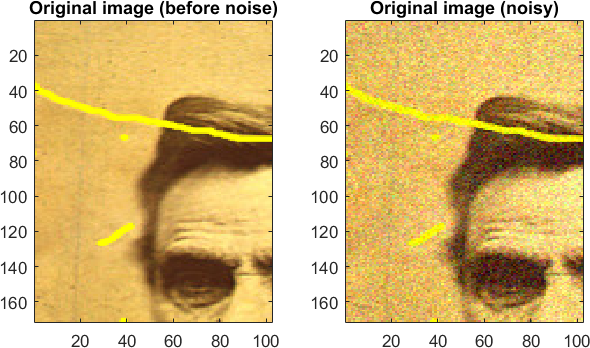
\includegraphics[width=0.7\textwidth]{lincoln_medium_original}
    \caption{Het originele beeld, voor en na toevoeging van ruis}
\end{subfigure}

\begin{subfigure}[b]{\linewidth}
	\centering
    \captionsetup{justification=centering}
    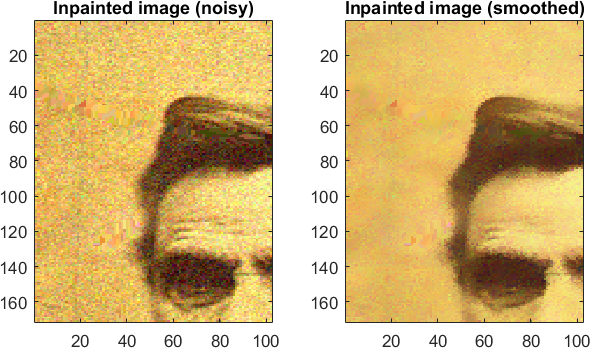
\includegraphics[width=0.7\textwidth]{lincoln_medium_msdsmoothed}
    \caption{Links: het ingepainte beeld volgens de gewijzigde formules uit sectie \ref{kandidaten}\\Rechts: Hetzelfde beeld na smoothing met een bilaterale filter}
\end{subfigure}

\begin{subfigure}[b]{\linewidth}
	\centering
    \captionsetup{justification=centering}
    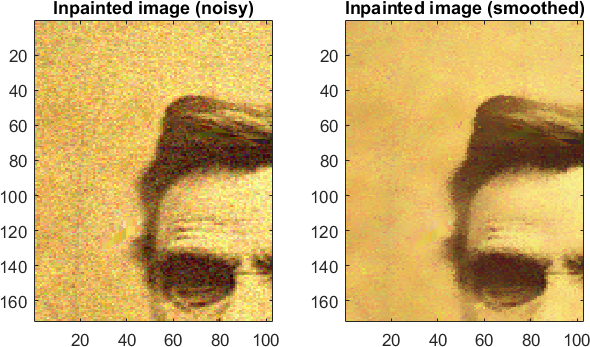
\includegraphics[width=0.7\textwidth]{lincoln_medium_unsmoothed}
    \caption{Links: het ingepainte beeld volgens de originele formules \ref{kandidaten}\\Rechts: Hetzelfde beeld na smoothing met een bilaterale filter}
\end{subfigure}
\caption{Een deel van het testbeeld \texttt{lincoln\char`_masked.png} (blokgrootte=25)} \label{fig:lincoln_medium}
\end{figure}

We pasten het algoritme van sectie \ref{kandidaten} dus aan zodat de pixels ingepaint worden met de uitgemiddelde waarde in plaats van de originele waarde. Dit heeft als nadeel dat de plaatsen waar ingepaint is vager zijn dan de rest van de afbeelding. Dit valt echter minder op dan de artefacten, en we behalen nu bijna soortgelijke resultaten als zonder ruisonderdrukking bij berekening van de MSD.

We blijven dus betere resultaten bekomen als we enkel ruisonderdrukking toepassen op de ingepainte afbeelding. Een verklaring hiervoor is dat het algoritme voor inpainting zonder aanpassingen zorgt dat de ingepainte regio zo sterk mogelijk op de omliggende regio's lijkt: deze zal dus ook ruis bevatten als er veel ruis is op de omliggende regio's en deze ruis zal ook gemakkelijker weggewerkt worden door de bilaterale filter. \\
Samenhang is in dit algoritme van belang: we krijgen minder goede resultaten als we de MSD bepalen vanuit een gefilterde versie van een afbeelding en bij het inpainten pixels te kopi\"eren vanuit een ongefilterde versie van de afbeelding (dit kan ervoor zorgen dat bepaalde ruispixels veel meer geselecteerd worden en de ruiswaarde dus gepropageerd wordt, waardoor we opvallende artefacten bekomen), en we krijgen minder goede resultaten als we een ongefilterde versie van een afbeelding inpainten gebaseerd op een gefilterde versie van de afbeelding (dit zorgt ervoor dat de ingepainte regio's duidelijk gefilterd zijn).

We kunnen echter nog steeds de afbeelding filteren gebaseerd op hoe onzeker het algoritme is over de ingepainte waarde. We kunnen een bepaalde pixel meer uitmiddelen op basis van het aantal onbekende pixels in de blok rond die pixel, of op basis van de iteratie waarin de pixel werd ingepaint (en dus hoeveel andere ingepainte pixels gebruikt werden om de waarde van de pixel te bepalen). Van dit laatste kan u een voorbeeld zien in Figuur \ref{fig:fence}.

\begin{figure}[H]
\centering
\begin{subfigure}[b]{\linewidth}
	\centering
    \captionsetup{justification=centering}
    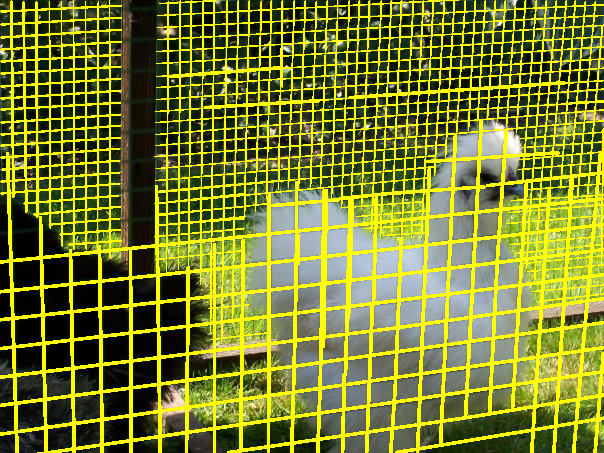
\includegraphics[width=0.45\textwidth]{fence_mask}
    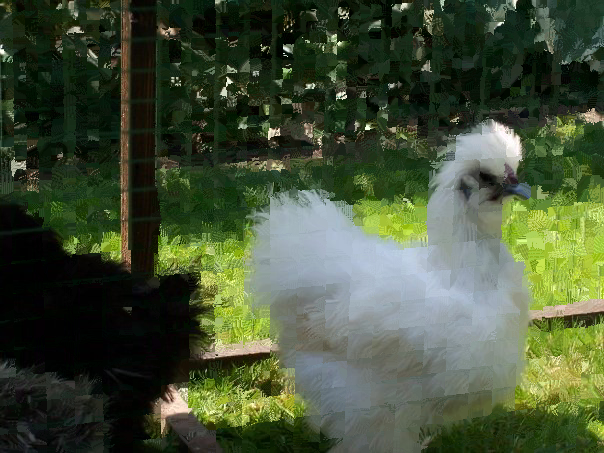
\includegraphics[width=0.45\textwidth]{fence_unsmoothed}
    \caption{Links: het originele beeld met masker\\Rechts: het ingepainte beeld voor smoothing. Het roosterpatroon is nog steeds duidelijk zichtbaar.}
\end{subfigure}

\begin{subfigure}[b]{\linewidth}
	\centering
    \captionsetup{justification=centering}
    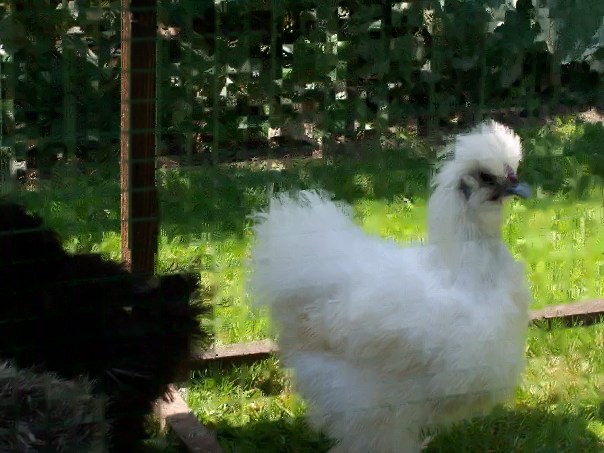
\includegraphics[width=0.9\textwidth]{fence_adaptive_iter}
    \caption{Het ingepainte beeld na adaptieve smoothing op basis van iteratie. Het roosterpatroon is minder zichtbaar dankzij adaptieve smoothing.}
\end{subfigure}
\caption{Een deel van het testbeeld \texttt{fence\char`_mask.png} (blokgrootte=4, zoekvenstergrootte=8)} \label{fig:fence}
\end{figure}

% subsection ruisonderdrukking_en_inpainting (end)
% section ruis (end)

\section{Toepassingen}
\subsection{Verwijderen van vlekken en krassen in oude films}
Het probleem van automatisch krassen detecteren is veel besproken in de literatuur, maar dit gaat vooral over \'e\'en soort  krassen, verticale krassen. Dit is omdat dit heel vaak voorkomt bij oude films die beschadigd geraken. Aangezien onze krassen niet enkel verticaal zijn gaan we de detectiemethodes meerdere keren toepassen, telkens op een afbeelding die iets meer gedraaid is.\\
De puntvlekken zijn niet zeer groot of opvallend en zullen niet gedetecteerd worden door voorgaande methode. We kunnen echter wel lichte ruisondrukking toepassen deze puntvlekken kwijt te raken.

De manier die wij gebruikt hebben is een aangepaste versie van deze besproken in \cite{scratch_detection} en bestaat uit twee stappen, eerst maken we een binair beeld waar edges, en dus ook krassen, op gemarkeerd staan. Als tweede stap passen we de Houghtransformatie toe om het aantal mogelijke kassen in te perken.\\
Om het uiteindelijke binair beeld te vormen maken we gebruik van twee binaire beelden die worden vergeleken met een logische OR. Het eerste beeld is verkregen via Canny edge detection en de tweede via de methode besproken in \cite{scratch_detection}, wij nemen echter het gemiddelde over 10 i.p.v. 3 pixels aangezien dit voor veel minder false positives zorgt.
Deze tweede methode maakt gebruik van gradient waarden tussen pixels. Voor elke pixel word de gemiddelde waarde genomen van de $x$ waarden boven, onder, links en rechts van deze pixel. Naast deze waarden wordt er ook nog gekeken naar de pixel boven, onder, links en rechts van de huidige pixel in het originele beeld. Al deze waarden worden in zes functies gegoten die dan a.d.h.v. van twee parameters, $\alpha$ en $\beta$, bepalen of de pixel in het binair beeld een 1 of een 0 zal zijn.\\
We nemen een combinatie van beiden afbeeldingen omdat Canny te veel edges aanduid en de in \cite{scratch_detection} besproken methode de edges niet duidelijk genoeg aanduid, dit is te zien op Figuur \ref{fig:edge_detection}. Een combinatie van beide blijkt in de praktijk beter te werken.\\
\begin{figure}[H]
  \centering
  \begin{minipage}{\textwidth}
    \centering
    \captionsetup{justification=centering}
    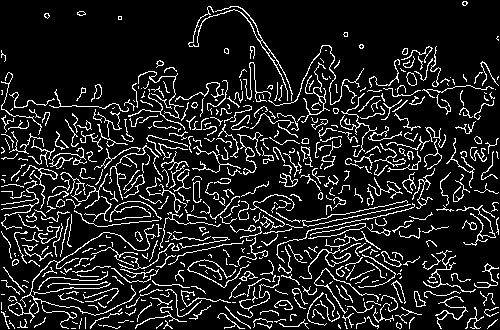
\includegraphics[width=.4\textwidth]{canny}\quad
    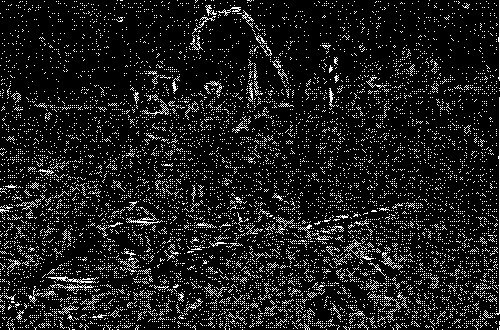
\includegraphics[width=.4\textwidth]{binary_img}\quad
    \subcaption{Links: Canny edge detection\\Rechts: Gradient edge detection}
  \end{minipage}\\[1em]
  \begin{minipage}{\textwidth}
      \centering
    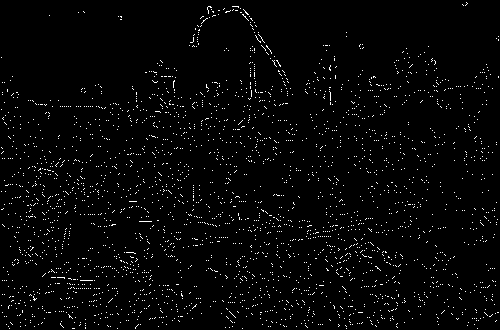
\includegraphics[width=.4\textwidth]{final_binary_img}
    \subcaption{Combinatie van Canny en Gradient}
  \end{minipage}
  \caption{Edge detection op \texttt{ww1\char`_original.png}} \label{fig:edge_detection}
\end{figure}

Hough transform kan lijnen detecteren die ongeveer verticaal staan, ze mogen +- 5$\deg$ gedraaid staan. Dit wil zeggen dat we de afbeelding op minstens $180/10=18$ hoeken moeten beschouwen, door wat te experimenteren bleek dit echter niet voldoende en was 24 een beter aantal. Voor elke hoek tekenen we de lijnen uit, in het wit, op een zwarte achtergrond en roteren die terug naar de originele positie. Deze afbeelding wordt dan gecombineerd met de al bestaande mask m.b.v. een logische OR, het resultaat ziet u op Figuur \ref{fig:mask}. Hierna passen we nog een dilatie toe omdat de gevonden lijnen niet de gehele kras bedekken.\\
Na de hough transform toe te passen hebben we nog steeds redelijk wat false positives. Deze zijn echter moeilijk te onderscheiden van echte krassen en die hebben we dus ook niet weggelaten. Als we ervan uitgaan dat de krassen in een niet druk gedeelte liggen, zoals de lucht in \verb|ww1_original.png| en niet in het drukke deel met de soldaten, dan zouden we deze false positives wel kunnen elimineren.

Het uiteindelijke resultaat ziet u in Figuur \ref{fig:result_ww1}.

\begin{figure}[!ht]
  \centering
  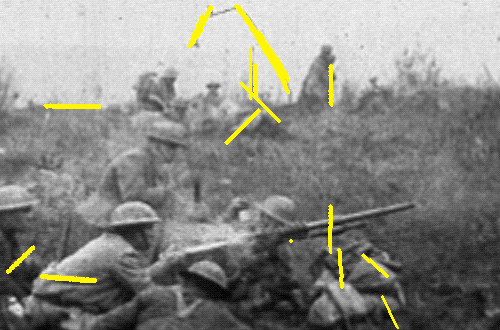
\includegraphics[width=.9\textwidth]{ww1_mask}
  \caption{Mask voor \texttt{ww1\char`_original.png}} \label{fig:mask}
\end{figure}

\begin{figure}[!ht]
  \centering
  \captionsetup{justification=centering}
  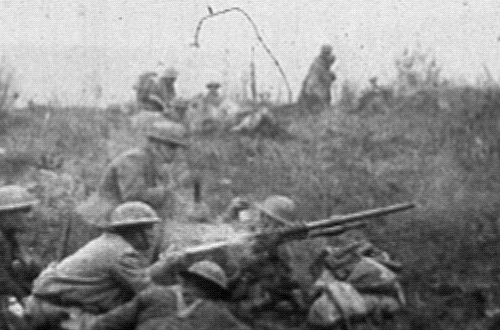
\includegraphics[width=.45\textwidth]{ww1_original}\quad
  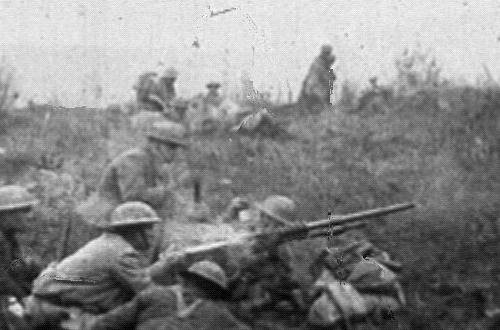
\includegraphics[width=.45\textwidth]{ww1_inpainted}  \caption{Inpainting na automatische krasdetectie op \texttt{ww1\char`_original.png}\\Links: het originele beeld\\Rechts: het ingepainte beeld} \label{fig:result_ww1}
\end{figure}
\FloatBarrier
\subsection{Verbergen van huizen in luchtfoto's}
In figuur \ref{fig:houses_erased} is het resultaat te zien van die algoritme op \textit{house\_erased}. 
Hierbij valt op dat op de plaats van de markering geen huis te herkennen is. Het algoritme heeft de vlek opgevuld, maar er zit geen structuur in pixels. De reden hiervoor is dat heel weinig informatie beschikbaar is over het in te vullen deel: het is een groot oppervlak met een relatief kleine omtrek, waardoor minder pixels nuttige informatie geven over de mogelijke ``inhoud'' van het vlak. ``Dunne'' markeringen kunnen gemakkelijk ingevuld worden door naar gelijkaardige blokken te zoeken, dit kan een goede schatting geven van wat er zou moeten staan. Wanneer echter een groot oppervlak moet ingevuld worden zouden heel grote blokken en zoekvensters moeten gebruikt worden waardoor het algoritme heel ineffici\"ent zou worden. In figuur \ref{fig:houses_erased_b} is het resultaat te zien voor het algoritme met de grootte van het zoekvenster gelijk aan 100 en blokgroote 40. In de figuur is duidelijk te zien dat een deel van de structuur gereconstrueerd is. Door de grote blokgrootte kan gezocht worden naar blokken waarbij de ``omgeving'' rond het in te vullen gebied gelijkaardig zijn. Het grote zoekvenster zorgt ervoor dat verder in de afbeelding naar een referentieblok kan worden gezocht. Samen leidt dit tot een soort patroonmatching die als referentieblok bijvoorbeeld een blok van een parallelle straat neemt omdat de omgeving gelijkend is (gras aan de ene kant, een straat aan de andere kant). Wel noemenswaardig is dat het algoritme 11 uur heeft gedraaid om dit resultaat te krijgen.
\par
Er is echter een andere, gelijkaardige oplossing die waarschijnlijk effici\"enter zou zijn. Aangezien we een volledig vlak moeten invullen waarvan slechts weinig pixels informatie zullen hebben in hun omliggend blok zou het beter zijn om een blok te kiezen die het volledige in te vullen gebied bevat en dan in de volledige afbeelding naar een refentieblok te zoeken. Eens dit gevonden is kunnen alle pixels van het in te vullen gebied in een iteratie opgevuld worden. Dit in contrast met de iteratieve methode waar voor elke ontbrekende pixel een referentieblok wordt gezocht. Hiermee wordt ook vermeden dat reeds ingepainte pixels als referentie zullen gebruikt worden. Voor kleine oppervlakken zou dit geen kwaad kunnen, maar voor grote gebieden zullen de ingevulde pixel weinig nuttige informatie bevatten, de kwaliteit van de informatie zal afnemen hoe centraler in het in te vullen gebied de ingepainte pixel ligt.

\begin{figure}[!ht]
    \centering
    \captionsetup{justification=centering}
    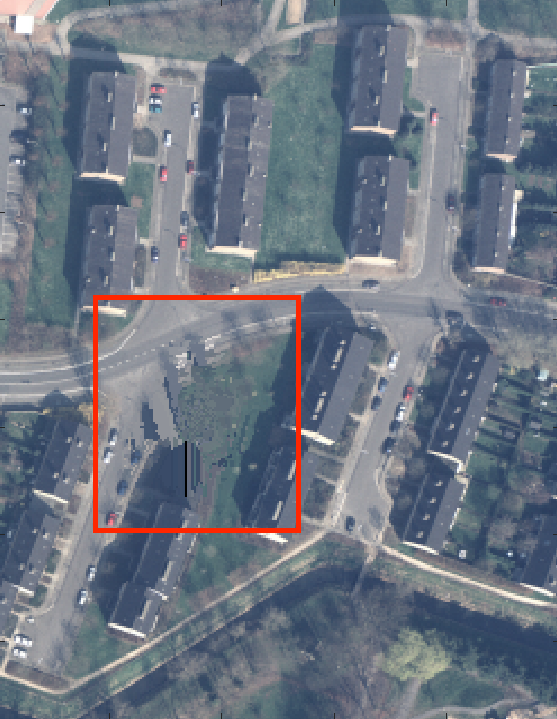
\includegraphics[width=.4\textwidth]{houses_erased_31_16}
    \quad
    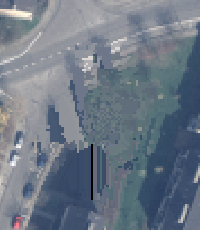
\includegraphics[width=.4\textwidth]{houses_erased_31_16_zoomed}
    \caption{Inpainting van \texttt{houses\_erased.png} met \texttt{SearchWindowSize}=31 en \texttt{BlockSize}=16. Links de volledige afbeelding, rechts een uitvergroting van het ingepainte gebied.} 
    \label{fig:houses_erased}
\end{figure}

\begin{figure}[!ht]
    \centering
    \captionsetup{justification=centering}
    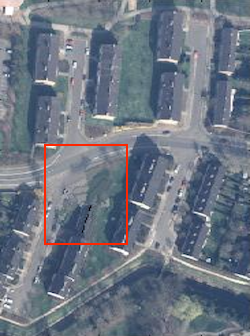
\includegraphics[width=.4\textwidth]{houses_erased_40_100}
    \quad
    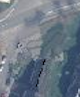
\includegraphics[width=.4\textwidth]{houses_erased_40_100_zoomed}
    \caption{Inpainting van \texttt{houses\_erased.png} met \texttt{SearchWindowSize}=100 en \texttt{BlockSize}=40. Links de volledige afbeelding, rechts een uitvergroting van het ingepainte gebied.} 
    \label{fig:houses_erased_b}
\end{figure}
\FloatBarrier
\subsection{Verwijderen van tekst in een beeld}
We voerden het programma uit op \texttt{houses\char`_text.png} met verschillende parameters. Op figuur \ref{fig:houses_text} zien we de twee beste resultaten resp. zonder en met ruis.

Het resultaat zonder ruis lijkt erg op het originele beeld. Op sommige plaatsen lijkt het beeld wat ruis te hebben terwijl de textuur van de omliggende gebieden vlak is. Het inpainting-algoritme zou dus verbeterd kunnen worden door rekening te houden met de textuur.\\
Het resultaat met ruis is duidelijk erg vervaagd maar lijkt nog steeds op het originele beeld. Er is natuurlijk altijd een trade-off tussen hoeveelheid ruis en vaagheid, maar dankzij het gebruik van een bilaterale filter blijven de randen toch grotendeels bewaard. Op het beeld voor ruisonderdrukking (hier niet afgebeeld) waren duidelijk meer artefacten te zien door de invloed van ruis op de MSD, maar deze zijn veel minder duidelijk te zien na ruisonderdrukking en zoals besproken in sectie \ref{ruisonderdrukking_en_inpaintig} zouden er meer sporen van inpainting achterblijven bij aanpassing van de berekening van de MSD.

\section{Besluit}
We kunnen concluderen dat gebruikte inpaintingtechniek (per ontbrekende pixel naar een referentieblok zoeken) geen ``silver bullet'' is. In sommige gevallen zal deze techniek zeer goed werken (bijvoorbeeld voor afbeeldingen waar een zekere textuur in zit die moet gereconstrueerd worden). Maar zelfs bij dit soort afbeeldingen zullen de parameters die optimale resultaten geven verschillend zijn. Voor andere afbeeldingen kunnen andere inpaintingtechnieken (bijvoorbeeld interpolatie) beter preseteren. Het combineren van verschillende technieken is ook een mogelijkheid. Als besluit kunnen we stellen dat de kwaliteit van deze inpaintingtechniek afhankelijk is van de afbeelding. Daarnaast kunnen we stellen dat de technieken die best toegepast kunnen worden voor reconstructie afhankelijk zijn van de eigenschappen van het beeld (foto, lijnen, egale vlakken, patronen, \ldots). Op basis van deze eigenschappen kunnen technieken gekozen en gecombineerd worden om een zo optimaal mogelijk resultaat te krijgen.

\begin{figure}[H]
  \centering
  \begin{minipage}{\textwidth}
    \centering
    \captionsetup{justification=centering}
    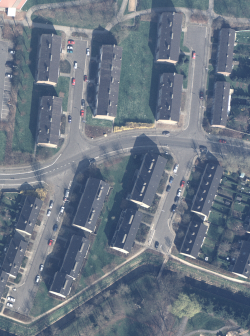
\includegraphics[width=.4\textwidth]{houses}\quad
    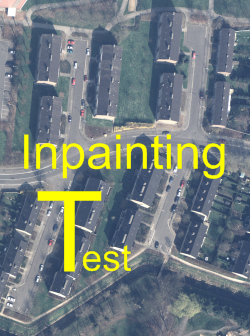
\includegraphics[width=.4\textwidth]{houses_text}
    \subcaption{Links: het originele beeld\\Rechts: het beeld na toevoeging van tekst}
  \end{minipage}\\[1em]
  \begin{minipage}{\textwidth}
    \centering
    \captionsetup{justification=centering}
    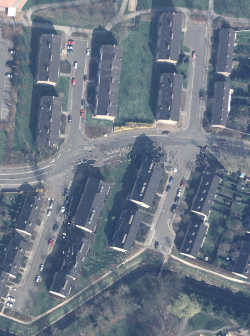
\includegraphics[width=.4\textwidth]{houses_clean_16_inpainted}\quad
    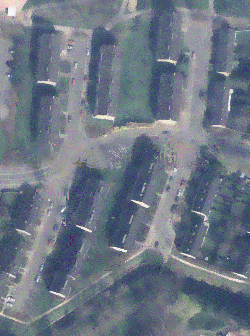
\includegraphics[width=.4\textwidth]{houses_noise_smoothed}
    \subcaption{Links: het ingepainte beeld zonder ruis (blokgrootte=16)\\Rechts: het ingepainte beeld na toevoeging van ruis en smoothing (ruisniveau=20)}
  \end{minipage}
    \caption{Inpainting van \texttt{houses\char`_text.png} met \texttt{SearchWindowSize}=31} \label{fig:houses_text}
\end{figure}

\begin{thebibliography}{1}
\bibitem{scratch_detection}
  S. Ghosh, R. Saha,
  "A Simple and Robust Algorithm for the Detection of
Multidirectional Scratch from Digital Images",
  Advances in Pattern Recognition (ICAPR), 2015 Eighth International Conference,
  pp. 1-6,
  Januari 2015.
\end{thebibliography}
\end{document}